\let\negmedspace\undefined
\let\negthickspace\undefined
\documentclass[journal]{IEEEtran}
\usepackage[a5paper, margin=10mm, onecolumn]{geometry}
%\usepackage{lmodern} % Ensure lmodern is loaded for pdflatex
\usepackage{tfrupee} % Include tfrupee package

\setlength{\headheight}{1cm} % Set the height of the header box
\setlength{\headsep}{0mm}     % Set the distance between the header box and the top of the text

\usepackage{gvv-book}
\usepackage{gvv}
\usepackage{cite}
\usepackage{amsmath,amssymb,amsfonts,amsthm}
\usepackage{algorithmic}
\usepackage{graphicx}
\usepackage{textcomp}
\usepackage{xcolor}
\usepackage{txfonts}
\usepackage{listings}
\usepackage{enumitem}
\usepackage{mathtools}
\usepackage{gensymb}
\usepackage{comment}
\usepackage[breaklinks=true]{hyperref}
\usepackage{tkz-euclide} 
\usepackage{listings}
% \usepackage{gvv}                                        
\def\inputGnumericTable{}                                 
\usepackage[latin1]{inputenc}                                
\usepackage{color}                                            
\usepackage{array}                                            
\usepackage{longtable}                                       
\usepackage{calc}                                             
\usepackage{multirow}                                         
\usepackage{hhline}                                           
\usepackage{ifthen}                                           
\usepackage{lscape}
\begin{document}

\bibliographystyle{IEEEtran}
\vspace{3cm}

\title{3-3.3-13}
\author{EE24BTECH11064 - Harshil Rathan}
% \maketitle
% \newpage
% \bigskip
{\let\newpage\relax\maketitle}

\renewcommand{\thefigure}{\theenumi}
\renewcommand{\thetable}{\theenumi}
\setlength{\intextsep}{10pt} % Space between text and floats


\numberwithin{equation}{enumi}
\numberwithin{figure}{enumi}
\renewcommand{\thetable}{\theenumi}
\textbf{Question}:\\
Draw a triangle $ABC$ in which $BC = 7cm$, and $\angle B = 45\degree$, $\angle{C}=60^\circ$.\\
\solution \\
\begin{table}[h!]
    \centering
    \begin{tabular}[12pt]{ |c| c|}
    \hline
    \textbf{Equations}& \textbf{Given}\\ 
    \hline
     $2y$ & $3x+12$ \\
    \hline 
     $x$ & $2, 8 $\\
    \hline
    \end{tabular}
    \caption{Given Equations}

\end{table}
Find $\angle{A}$
\begin{align}
     \angle{A}+\angle{B}+\angle{C}=180^\circ 
\end{align}    
\begin{align}    
     \angle{A}=75^\circ
\end{align}
Using the Sine Rule,
\begin{align}
    \frac{a}{\sin{A}}=\frac{b}{\sin{B}}=\frac{c}{\sin{C}}
    \label{0.3}
\end{align}
\begin{align}
    b=\frac{a \sin B}{\sin A} 
\end{align}
\begin{align}
    b=\frac{14\sqrt{2}}{\sqrt{6}+\sqrt{2}}
    \label{0.5}
\end{align}
\begin{align}
    c=\frac{a \sin C}{\sin A}
\end{align}
\begin{align}
      c= \frac{14\sqrt3}{\sqrt6+\sqrt2}
      \label{0.7}
\end{align}
Therefore measure of the sides are, \ref{0.5} \ref{0.7} \\
$AB=7.06cm$ , $BC=7cm$ , $CA=9cm$
\begin{figure}[h!]
   \centering
   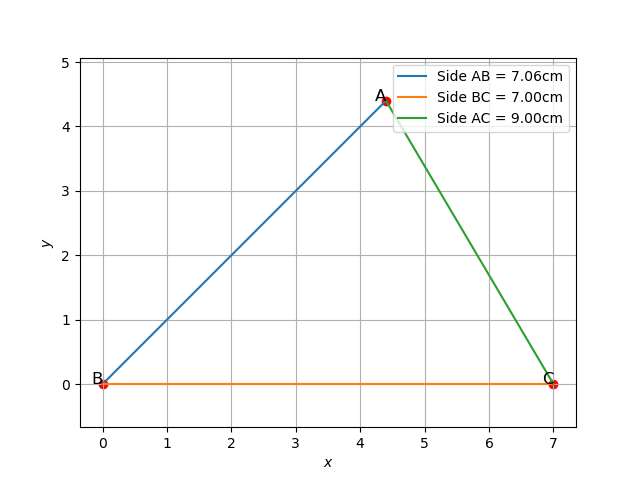
\includegraphics[width=\linewidth]{figs/Figure_1.png}
   \caption{}
   \label{stemplot}
\end{figure}





\end{document}
